\subsection{Logical View}

\copied{Logical view : The logical view is concerned with the functionality that the system provides to end-users. UML Diagrams used to represent the logical view include Class diagram, Communication diagram, Sequence diagram.[2]}
{from wikipedia\\\url{https://en.wikipedia.org/wiki/4\%2B1_architectural_view_model}}

This view shows the structural elements, key abstractions and mechanisms that are used within HPS to realize the systemics functionality. At first an overview of the components is provided. After that the main components are decomposed and desired in term of responsibilities and interfaces. In the end, the variability guide mentions parts of the software, which clarification is deferred until development/design phase.

%Used algorithms?:
%	hidden markov model with k means (unsupervised learning)
%	Singular Spectrum Analysis (SSA) for locations with tides?
%	“limit checking”
%	
%	Gauss-Markov
%	Something with correlation? https://en.wikipedia.org/wiki/Cross-correlation? Thesis zecht te kijken naar:
%	[74] Logan, D., Mathew, J. Using the Correlation Dimension for Vibration Fault
%Diagnosis of Rolling Element Bearing – I. Basic Concepts, Mechanical Systems and
%Signal Processing, Vol. 10, No. 3, pp. 241-250, (1996)
%[75] Logan, D., Mathew, J. Using the Correlation Dimension for Vibration Fault
%Diagnosis of Rolling Element Bearing – II. Selection of Experimental Parameters,
%Mechanical Systems and Signal Processing, Vol. 10, No. 3, pp. 251-264, (1996)

\clearpage
\begin{figure}[hb!]
%\centering
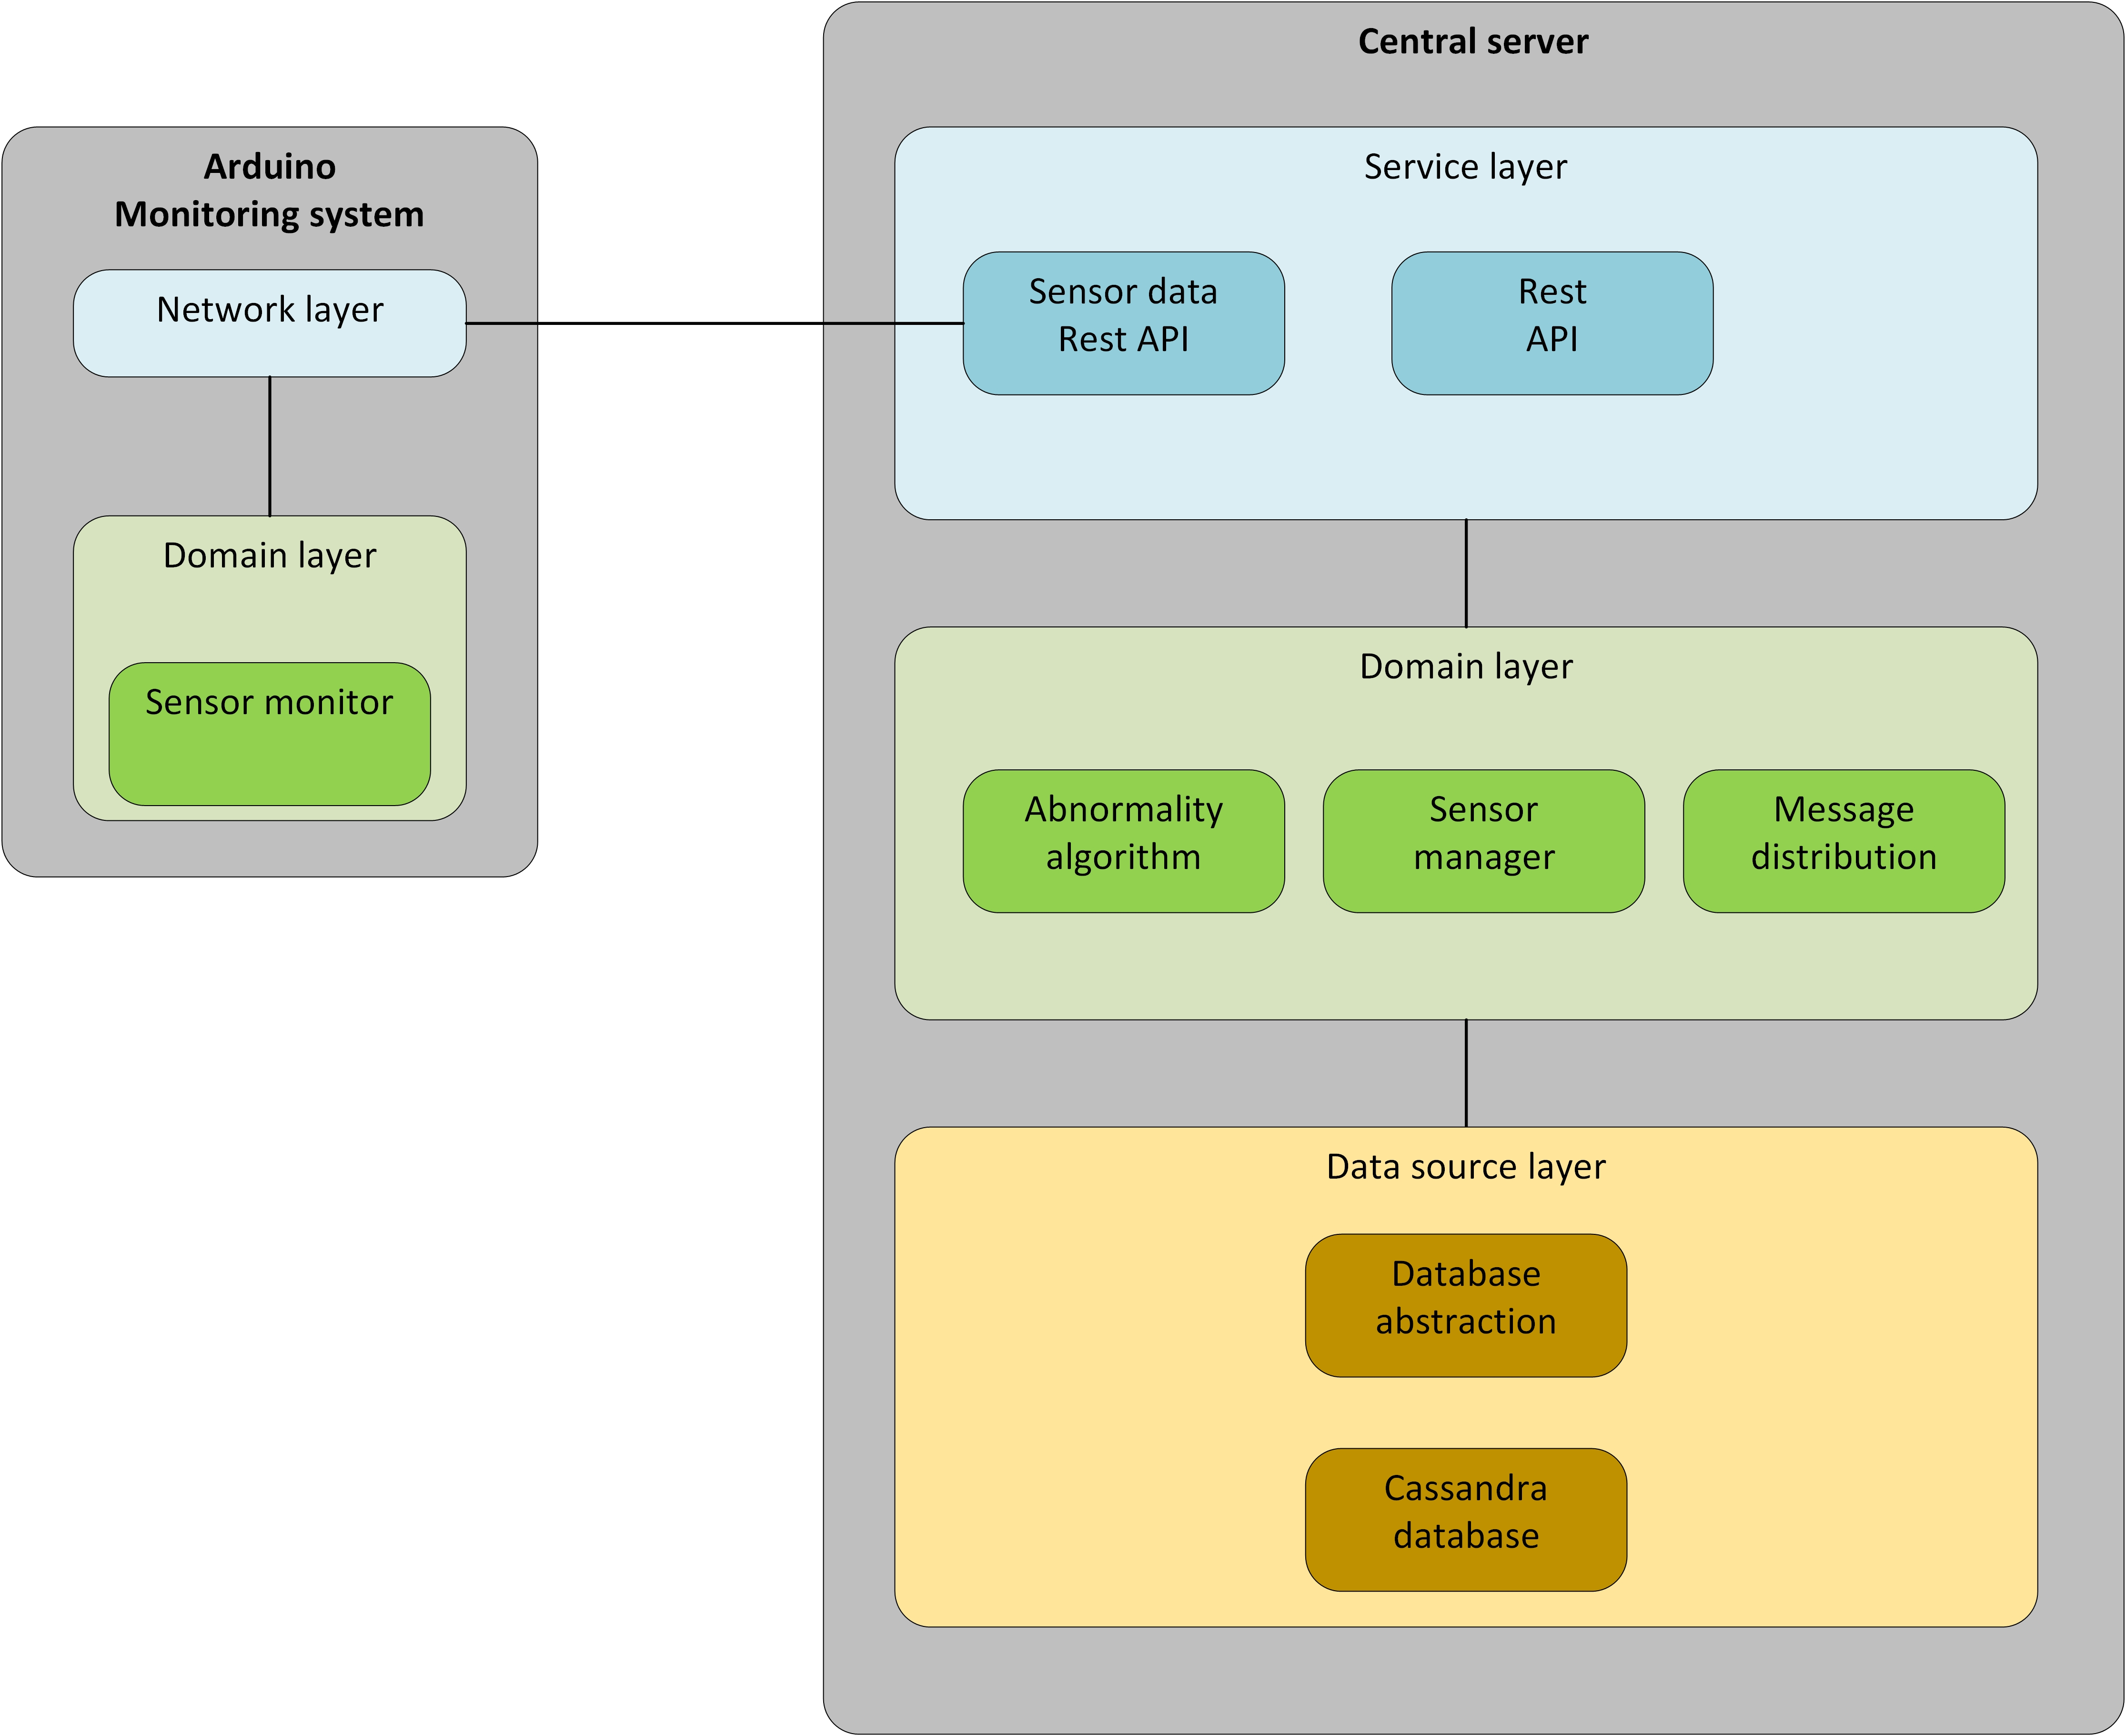
\includegraphics[keepaspectratio=true,width=0.9\textwidth]{{\viewimages/layers}.jpg}
\caption{Layers of the software}
\label{fig:layers}
\end{figure}

\clearpage
\begin{figure}[h]
%\centering
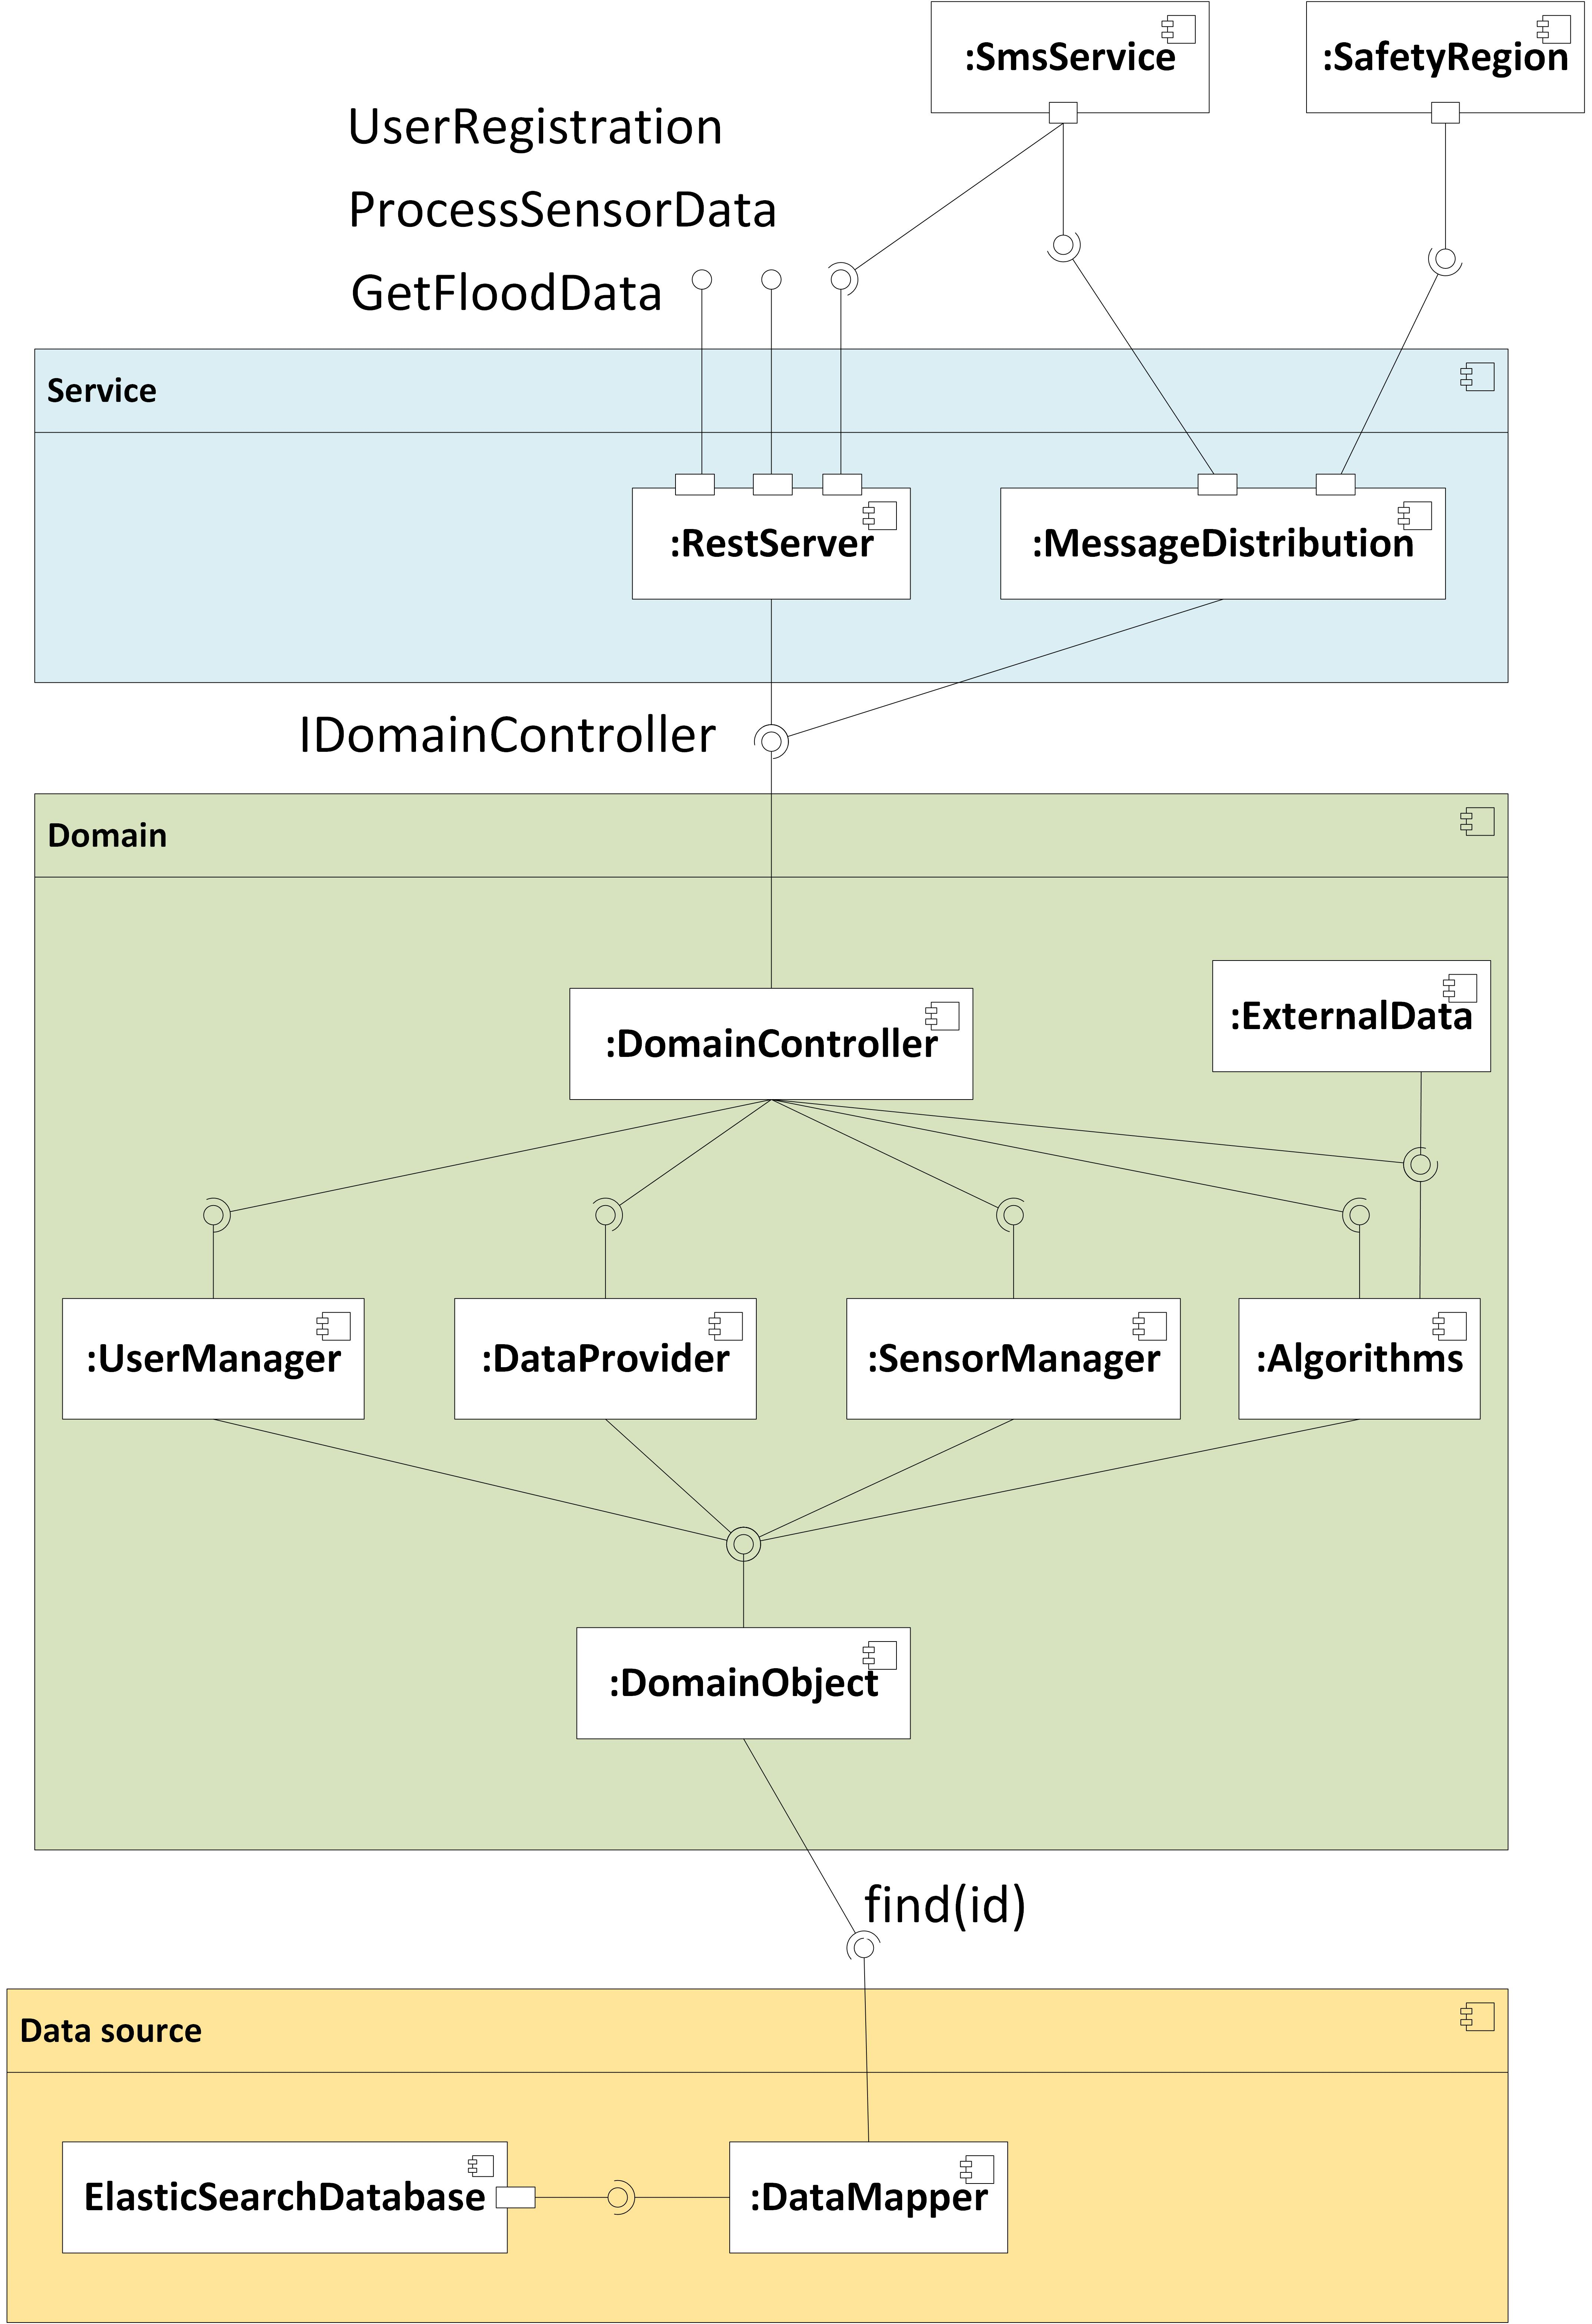
\includegraphics[keepaspectratio=true,width=0.9\textwidth]{{\viewimages/component}.jpg}
\caption{Component diagram}
\label{fig:component}
\end{figure}

\begin{figure}[hb!]
%\centering
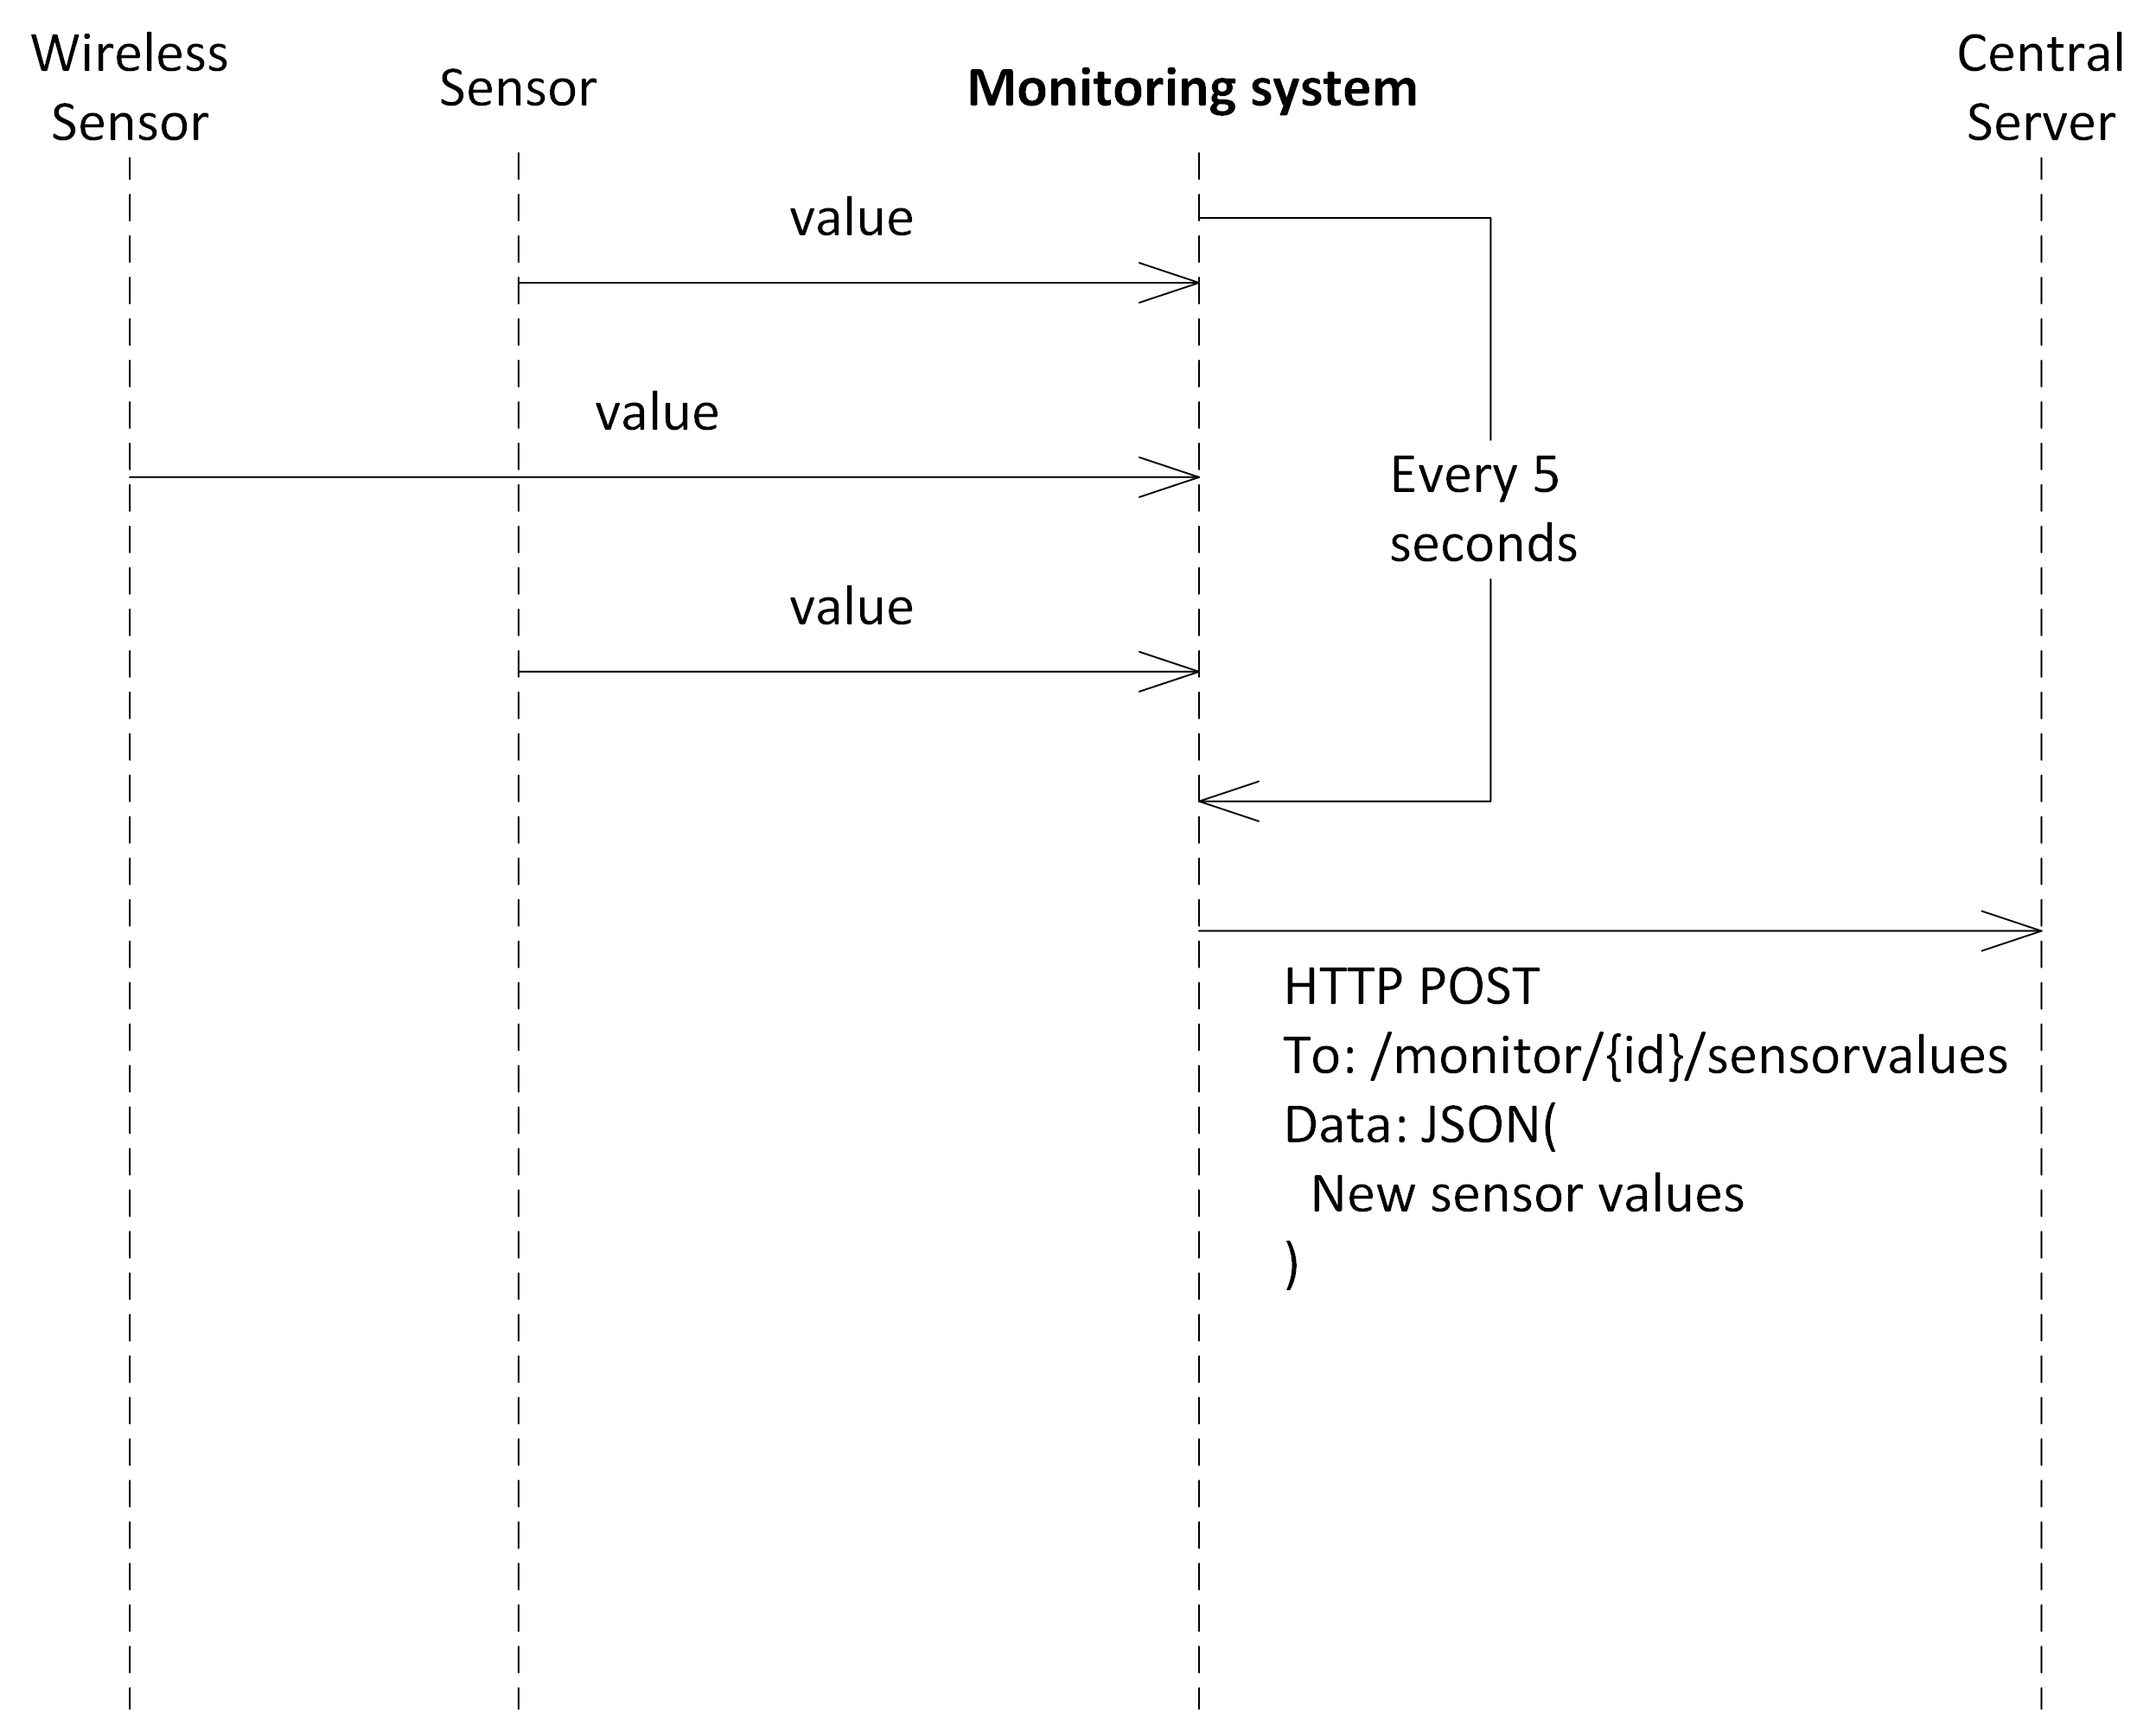
\includegraphics[keepaspectratio=true,width=0.9\textwidth]{{\viewimages/sequence1}.jpg}
\caption{Sequence diagram of the client pushing the sensor data}
\label{fig:component}
\end{figure}

\clearpage
\begin{figure}[hb!]
%\centering
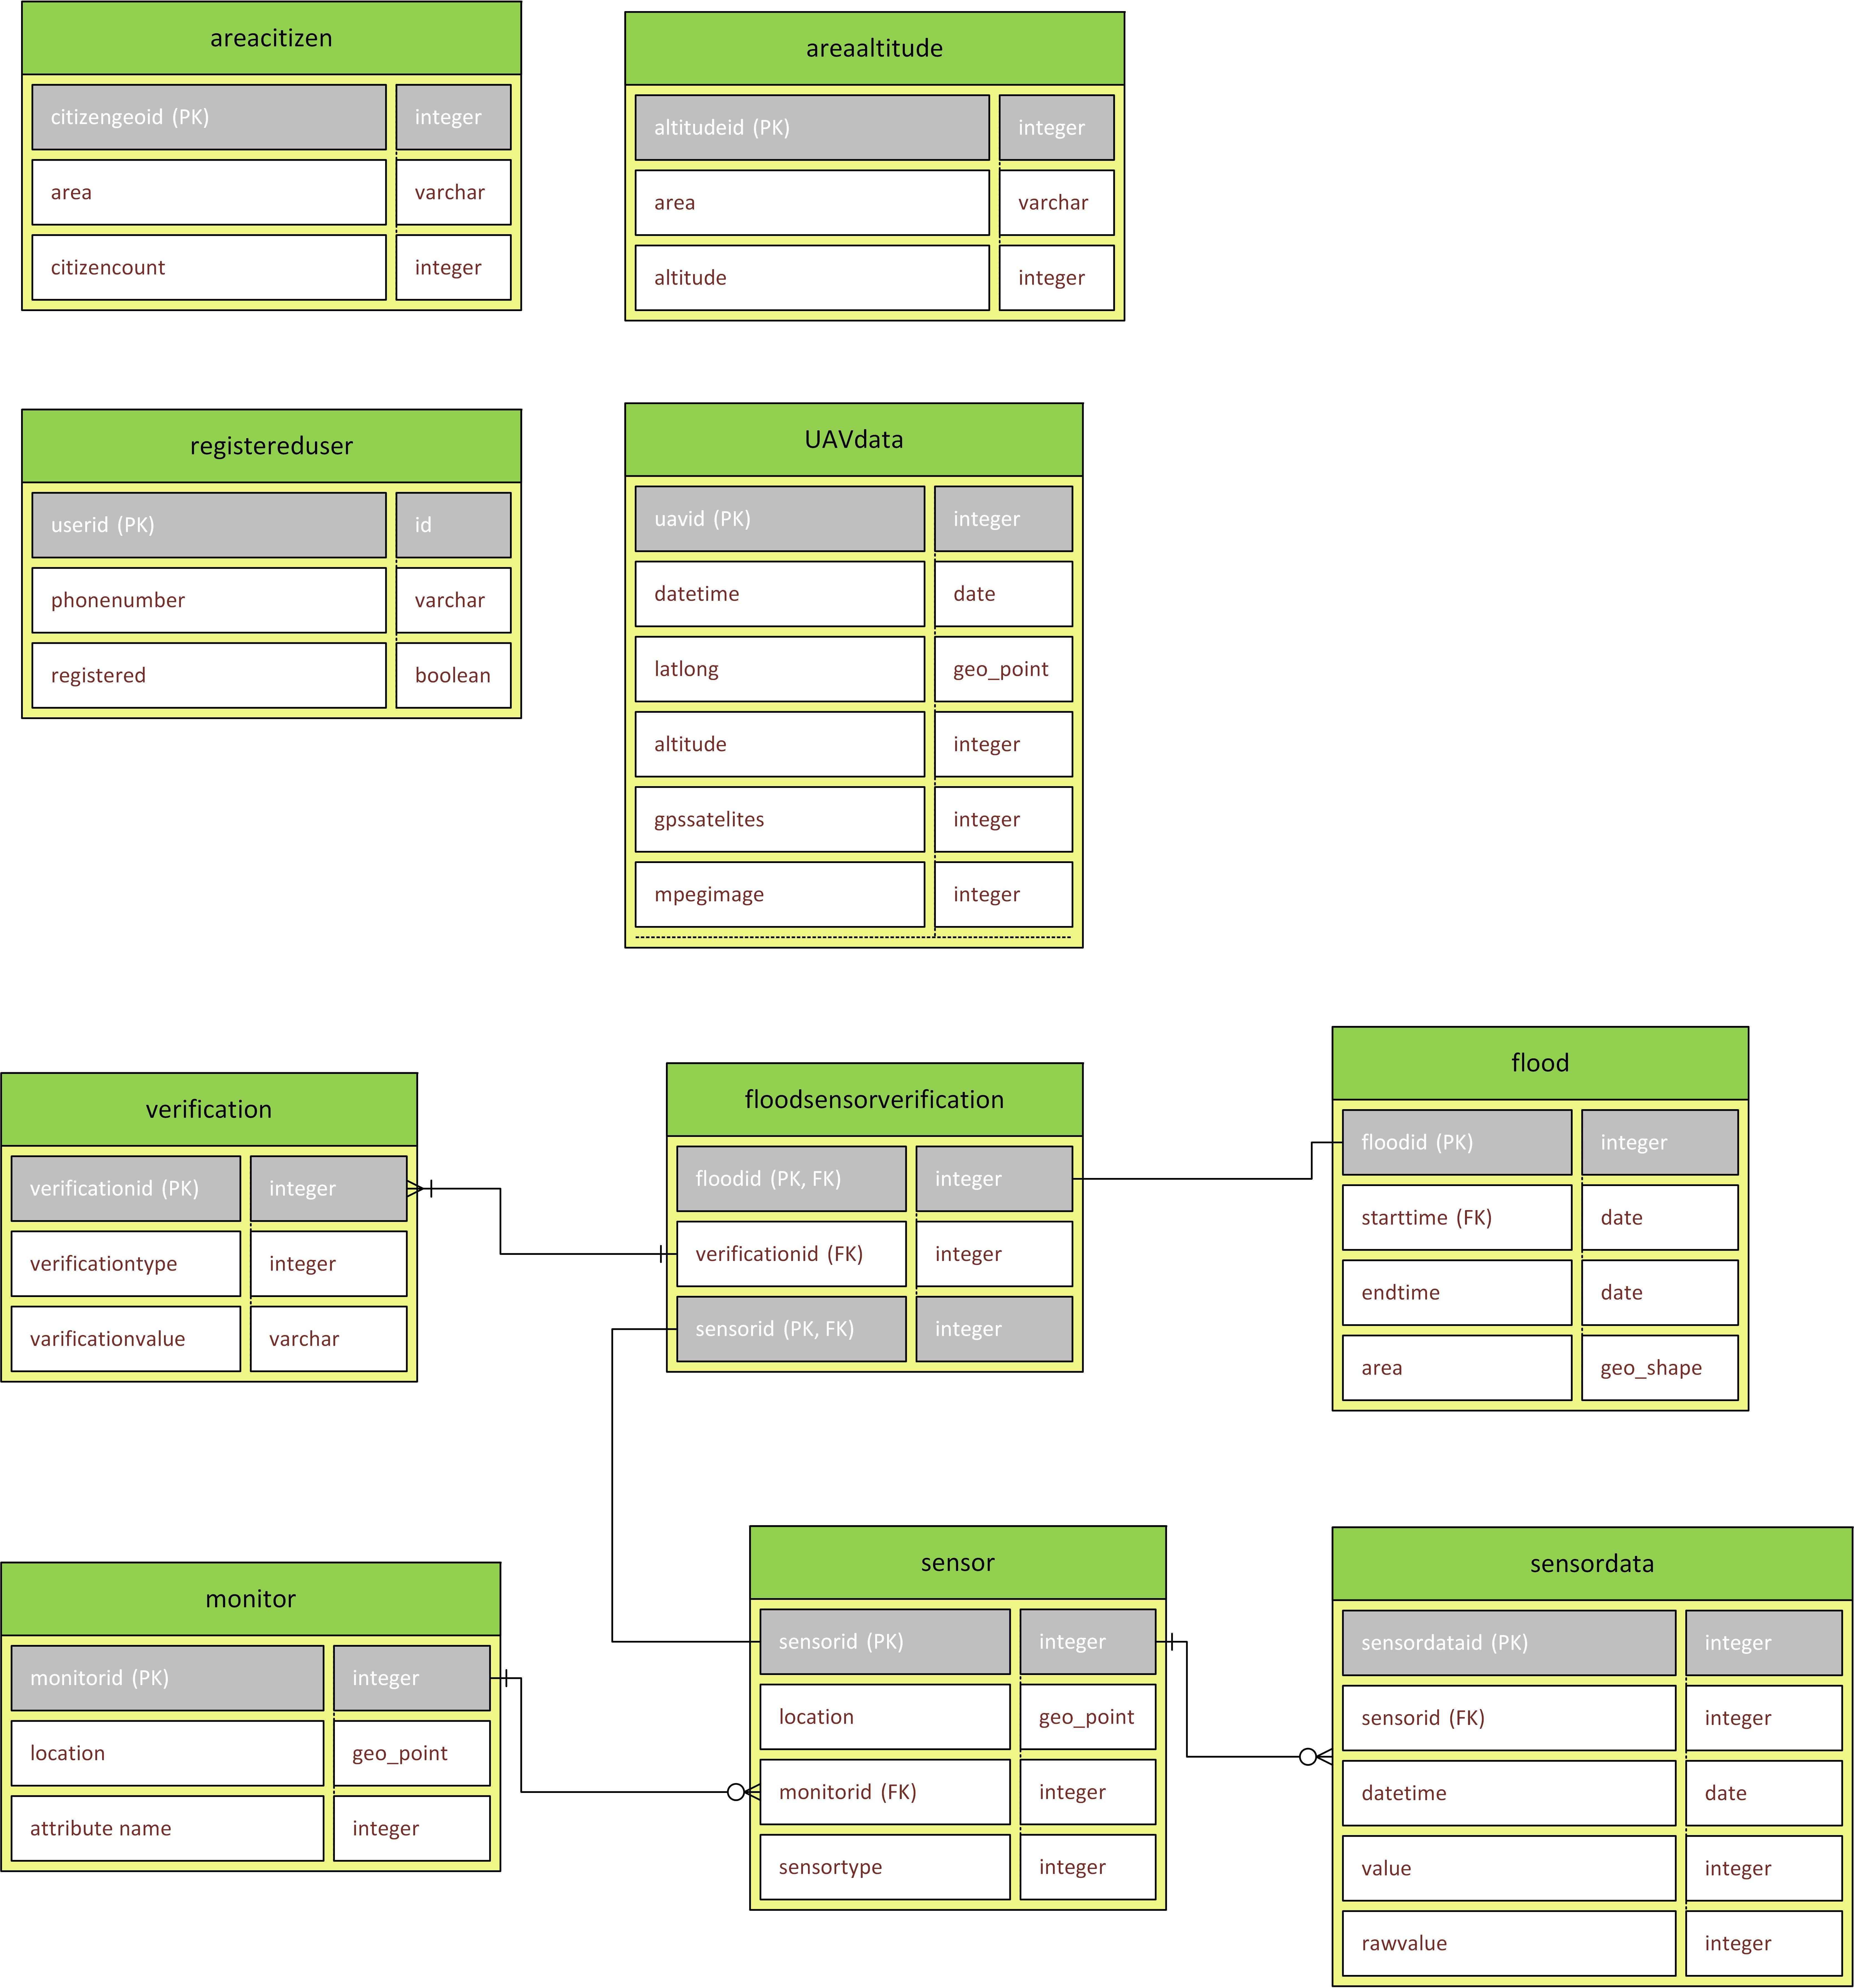
\includegraphics[keepaspectratio=true,width=0.9\textwidth]{{\viewimages/database}.jpg}
\caption{Database diagram}
\label{fig:component}
\end{figure}

%\begin{framed}
%
%	Update monitor system firmware? Do we do this? And how do we do this?
%	Do sensors have firmware and how do we update that?
%
%\end{framed}

